\documentclass[a4paper, 12pt]{scrartcl}



\usepackage[utf8]{inputenc}

\usepackage[ngerman]{babel}
\usepackage{amssymb}
\usepackage[T1]{fontenc}
\usepackage{mathtools}
\usepackage{amsmath}
\usepackage{ntheorem}
\usepackage{bbm}
\usepackage{dsfont}
\usepackage{color}
\usepackage{slashed}
\usepackage{hyperref}
\usepackage{graphicx} 
\usepackage{bm}
\usepackage{mathabx}
\usepackage{multirow}
\usepackage{float}
\usepackage{mwe}
\begin{document}
\begin{titlepage}
	\centering
	{\scshape\LARGE Universität Tübingen \par}
	\vspace{2cm}
	{\huge\bfseries Ultraschall \par}
	\vspace{2cm}
	{\Large \scshape Blockpraktikum 2021} \par
	\vspace{2cm}
	{\Large  Erste korrigierte Version} \par
	\vspace{2cm}
	{\Large\itshape \underline{David Schütz} \space \space  \underline{Christian Gommeringer}\par}
	\vfill 
	{\large unter Betreuung von Ivan Musil}
	\vfill

	{\large \today\par}
\end{titlepage}
\newpage 
\tableofcontents 
\vfill
\noindent\rule[1ex]{\textwidth}{0.25pt}
\newpage
\section{Einleitung}
\begin{flushleft}
In dieser kleinen Versuchsreihe aus drei Versuchen untersuchen wir die Ausbreitung von Ultraschallwellen in verschiedenen Medien und dessen Auswirkungen. Zunächst bedarf es jedoch einer Einführung in die theoretischen Grundlagen der Versuche und danach erfolgt die Erklärung der Versuche und dessen Ausführung. Abschließend werden wir die drei Versuche auswerten und präsentieren und ein Resümee ziehen was wir in den Versuchen gelernt haben. 
\end{flushleft}

\vfill
\noindent\rule[1ex]{\textwidth}{0.25pt}
\newpage
\section{Theoretische Grundlagen}  
\subsection{Die elastischen Koeffizienten}
Die Ausbreitung von Schallwellen basiert auf der elastischen Verformung des Ausbreitungsmediums. Um das genauer zu charakterisieren führt man die elastischen Koeffizienten ein. Eine genaue Darstellung zur Veranschaulichung der vier elastischen Koeffizienten findet sich in der Anleitung zum Versuch. Zum einen definiert man den \textbf{Elastizitätsmodul} $E$ als 
\begin{align}
E:= \frac{\sigma}{\epsilon} = \frac{F / A}{\Delta \ell / \ell}
\end{align}
mit der Normalspannung $\sigma$ und der Dehnung $\epsilon$. $\Delta \ell / \ell$ ist die relative Längenänderung. Weiter benötigen wir den \textbf{Schubmodul} $G$, der definiert ist als 
\begin{align}
G:= \frac{\tau}{\tan(\gamma)} \approx \frac{F / A}{\gamma}
\end{align}
mit der Schubspannung $\tau$ und dem Schubwinkel $\gamma$. (Hier wurde $\tan(\gamma)\approx \gamma$ genähert) Unter anderem benötigen wir weiter den \textbf{Kompressionsmodul} $K$, der definiert ist als 
\begin{align}
K:= - \frac{p}{\Delta V / V} 
\end{align}
mit dem Druck $p$ und der relativen Volumenänderung $\Delta V / V$. Zuletzt definieren wir noch die \textbf{Querkontraktionszahl} $\nu$ als 
\begin{align}
\nu := -\frac{\Delta d / d }{\Delta \ell / \ell}  
\end{align}
mit der relativen Dickenänderung $\Delta d / d$ und der relativen Längenänderung $\Delta \ell / \ell$. Sie ist dimensionslos und verknüpft die elastischen Koeffizienten miteinander durch 
\begin{align*}
E = 2(1+\nu)G = 3 (1-2\nu)K
\end{align*}
\subsection{Schallwellen}
Es gibt zwei Arten von Wellen im Medium. Bei Transversalwellen schwingt die sich fortpflanzende Größe, senkrecht zur Ausbreitungsrichtung, wobei sie bei Longitudinalwellen in Ausbreitungsrichtung schwingt. Ein Beispiel für Longitudinalwellen sind gewisse Schallwellen in Medien, bei denen die Teilchen parallel zur Ausbreitungsrichtung in ihrem rückstellenden Potential schwingen. Die Schallgeschwindigkeit der Longitudinalwellen in Flüssigkeiten und Gasen ist gegeben durch
\begin{align}
c_\textrm{L} = \sqrt{\frac{K}{\rho}} 
\end{align}
mit der Dichte $\rho$. In Festkörpern treten Transversal- und Longitudinalwellen auf, aufgrund des endlichen Schubmoduls. Die Schallgeschwindigkeiten sind 
\begin{align}
c_\textrm{L} = \sqrt{\frac{1-\nu}{1-\nu-\nu^2}  \frac{E}{\rho}} \approx \sqrt{\frac{E}{\rho}} \qquad c_\textrm{T} = \sqrt{\frac{G}{\rho}} = \sqrt{\frac{1}{2(1+\nu)} \frac{E}{\rho}}
\end{align}
dabei gilt stets $c_\textrm{L} \geq \sqrt{E/\rho} > \sqrt{G/\rho} = c_\textrm{T}$. 
\subsection{Debye-Sears-Effekt} 
Im ersten Versuchsteil haben wir eine besondere Anordnung. Es trifft eine Lichtwelle auf ein flüssiges Medium, in dem sich eine Schallwelle ausbreitet. Die Schallwelle induziert Dichteunterschiede im Medium und da die Ausbreitung von Licht von der Dichte abhängt, wirkt die sich ausbreitende Schallwelle wie ein Phasengitter und es entsteht ein Beugungseffekt am Schirm, der als Debye-Sears-Effekt bezeichnet wird. Die Erklärung für Phasengitter findet sich im entsprechenden Abschnitt \glqq Beugungsgitter \grqq .
\subsection{Beugung am Gitter}
Trifft kohärentes Licht einer bestimmten Wellenlänge ($\lambda_\text{Laser}$ auf einen Interferenzspalt mit einer Spaltbreite im Größenbereich der Wellenlänge selbst, wissen wir, dass auf dem dahinter zu beobachteten Schirm ein Beugungsmuster entsteht mit Maxima und Minima. Dies wird auch im ersten unserer Versuche eine Analogie sein, denn wir dürfen hier die gewöhnlichen Formel wie beim Beugungsgitter verwenden, wenn das Licht an der Schallwelle gebeugt wird, wie es beim Debye-Sears-Effekt passiert. Man erhält Intensitätsmaxima unter den Winkeln $\varphi_k$ zur optischen Achse, die die Bedingung erfüllen
\begin{align}
\sin(\varphi_k) = \frac{k \lambda_{\textrm{Laser}}}{g} \qquad k=0,1,2,...
\end{align}
wobei $g = \lambda$ entspricht, der Wellenlänge der Ultraschallwelle. Es gilt unter anderem die Kleinwinkelnäherung aufgrund des großen Schirmabstandes $d$ ($d\gg x_k$ , $x_k$ ist Abstand zweier Maxima) mit 
\begin{align}
\tan(\varphi_k) = \frac{x_k}{d} \cong \sin(\varphi_k)
\end{align}
\subsection{Beugungsgitter}
Ein Phasengitter ist ein Beugungsgitter, welches die Phase der durchlaufenden Lichtwelle beeinflusst. Sie sind im idealfall durchsichtig. Oft sind sie so konzipiert, dass an den Gitterstegen variierende Brechungindizes vorliegen oder eine variierende Materialstärke. Sie wirken sich nicht auf die Amplitude des Lichtes aus. \newline
\newline 
Im Gegenzug ist das Amplitudengitter ein Beugungsgitter, welches die Amplitude abschwächt durch regelmäßig angeordnete Bereiche, wie zum Beispiel lichtundurchlässige Streifen. Am Gitter ergibt sich dann eine periodische Amplitudenverteilung.   
\subsection{Snellius´sches Brechungsgesetz}
Beim Snellius´schen Brechungsgesetz stellt man sich zwei aneinanderliegende Medien vor mit Brechzahlen $n_1$ und $n_2$. Es trifft die Lichtwelle mit dem Auftreffwinkel $\delta_1$ ein und wird mit einem Austrittswinkel $\delta_2$ reflektiert oder auch gebrochen. Es formuliert sich als 
\begin{align}
n_1 \sin(\delta_1) = n_2 \sin(\delta_2)
\end{align}
Totalreflektion tritt dabei auf wenn der Auftreffwinkel folgendes erfüllt
\begin{align}
\delta_1 > \arcsin\left( \frac{n_2}{n_1} \right) 
\end{align}
\subsection{Piezo-Effekt}
Was zum Verständnis des Versuchs auch relevant sein mag, ist der Piezo-Effekt. Er beschreibt die Änderung der elektrischen Polarisation und somit das auftreten einer elektrischen Spannung an Festkörpern, wenn sie elastisch verformt werden. Beim inversen Piezoeffekt verursacht ein externes elektrisches Feld eine Verformung der Einheitszelle und somit eine Gesamtverformung des Piezokristalls.
\subsection{Magnetostriktion}
Bei der Magnetostriktion werden magnetische Stoffe deformiert durch anlegen eines magnetischen Feldes. Ferromagneten zeigen Domänen gleicher Magnetisierung die man als Weiss´sche Bezirke bezeichnet. Legt man ein äußeres Magnetfeld an werden die Weiss'schen Bezirke ausgerichtet. Das verursacht eine mechanische Verspannung des Materials und induziert somit eine Längenänderung in Magnetfeldrichtung. Die Magnetostriktion kann sowohl eine Ausdehnung, wie es z.B. bei Stahl der Fall ist, als auch eine Verkürzung, wie beispielsweise bei Nickel, bewirken. Diese Effekte werde auf natürliche Weise als positive und negative Magnetostriktion bezeichnet. Der Nickelstab, der in unserem Experiment untersucht wird, erfährt dabei bei konstantem Volumen eine elastische Längenänderung, die im $\mu$m-Bereich liegt.
\subsection{Schwingung eines Stabes}
Im ersten Versuch schwingt ein Stab mit einem festen und einem freien Ende. Die Wellenlänge $\lambda_k$ und die Länge des Stabes sind dabei verknüpft durch 
\begin{align}
\ell = (2k+1)\frac{\lambda_k}{4}
\end{align}
mit $k=0$ der Grundschwingung und $k=1$ der ersten Oberschwingung usw. Es folgt mit $\lambda_k=\frac{c_\textrm{L}}{f_k}$ und $c_\textrm{L} \approx \sqrt{E/\rho}$ für die Eigenfrequenz 
\begin{align}
f_k\approx  \frac{2k+1}{4\ell} \sqrt{\frac{E}{\rho}}
\end{align}
\subsection{Elastische Verformung}
Im zweiten Versuch untersuchen wir die elastische Verformung $\epsilon$ die gegeben ist durch 
\begin{align}
\epsilon = \frac{\Delta \ell}{\ell} = \kappa \Gamma \cdot \frac{H}{E}
\end{align}
dabei ist $H$ die magnetische Feldstärke und $E$ das Elastizitätsmodul. $\kappa \Gamma$ ist die Magnetostriktionskonstante. $H = NI /L$, wobei $I$ der Strom durch die Spule mit einer Anzahl von $N$ Windungen ist. Die Länge der Spule wurde mit $L$ bezeichnet. Es ergibt sich durch umstellen eine Steigung.
\begin{align}
m = \kappa \Gamma \cdot \frac{N \ell}{E L}
\end{align}
$N , L$ sind dabei die Materialkonstanten der Spule und $\ell$ die Länge des Stabes. Wir tragen später die Längenänderung als Funktion der Stromstärke auf und die Steigung wird uns da nützlich sein. 
\subsection{Geschwindigkeiten von Wellen}
Im letzten Versuch ist es noch notwendig die Geschwindigkeit von Longitudinalwelle und Transversalwelle zu errechnen. Die Gegebenheiten des Versuches und die Erkenntnis des Snellius´schen Gesetzes lässt ableiten, dass folgende Beziehung gilt
\begin{align}
\frac{\sin(\alpha)}{\sin(\beta_\textrm{L})} = \frac{c_\textrm{W}}{c_\textrm{L}}
\end{align}  
und auch 
\begin{align}
\frac{\sin(\alpha)}{\sin(\beta_\textrm{T})} = \frac{c_\textrm{W}}{c_\textrm{T}}
\end{align}
mit Einfallswinkel $\alpha$, Schallgeschwindigkeit in Wasser $c_\textrm{W}$, Brechwinkel $\beta_\textrm{L}$ und Schallgeschwindigkeit $c_\textrm{L}$ jeweils beides für die Longitudinalwelle und analog für die Transversalwelle der Brechwinkel $\beta_T$ und die Schallgeschwindigkeit $c_\textrm{T}$. Die Longitudinalwelle verschwindet bei Totalreflektion, also $\beta_\textrm{L}=90^\circ$ und einem Einfallswinkel $\alpha = \alpha_\textrm{L}$, und die Transversalwelle erreicht ihr Maximum bei $\beta_T = 45^\circ$ bei einem Einfallwinkel $\alpha = \alpha_T$. Es folgt mit Vereinfachung 
\begin{align}
c_\textrm{L} = \frac{c_\textrm{W}}{\sin(\alpha_\textrm{L})} \qquad \qquad c_\textrm{T} = \frac{c_\textrm{W}}{\sqrt{2} \sin(\alpha_\textrm{T})} 
\end{align} 
Bildet man das Verhältnis ergibt sich in Kombination mit den Gleichungen aus (6)
\begin{align}
\frac{c_\textrm{L}}{c_\textrm{T}} = \sqrt{\frac{2(1-\nu)}{1-2\nu}}
\end{align}
Anschließendes umstellen nach der Querkontraktionszahl $\nu$ ergibt letztlich 
\begin{align}
\nu = \frac{\frac{1}{2} \left( \frac{c_\textrm{L}}{c_\textrm{T}} \right)^2 -1 }{\left( \frac{c_\textrm{L}}{c_\textrm{T}} \right)^2-1}
\end{align}
\newpage
\section{Versuche}
\subsection{Versuch 1}
Im ersten Versuch wird mit einem Piezoquarz eine Ultraschallwelle in einem Ethanol gefüllten Behälter erzeugt und senkrecht mit einem kollimierten Laser ($\lambda_{\textrm{Laser}} = 632,8$nm) bestrahlt. Die Ultraschallwelle in der Flüssigkeit stellt eine elastische Welle dar mit regelmäßigen Abständen mit Bereichen von Über- und Unterdruck die nacheinander laufen. Die Flüssigkeit hat in Ausbreitungsrichtung der Schallwelle eine periodisch veränderliche Dichte und damit einen periodisch veränderlichen Brechungsindex und wirkt somit als Phasengitter.
Es wird jeweils fünf mal die erste und zweite Resonanzfrequenz gemessen, indem wir die Frequenz verändern und am Schirm schauen, wann das Beugungsbild am deutlichsten ist. Weiter stellen wir später die zweite Resonanzfrequenz $f_1$ ein und vermessen das Beugungsbild. Eine Darstellung unserer Ergebnisse findet der Leser unter \glqq Auswertung 1\grqq .
 
\subsection{Versuch 2} 
Im zweiten Versuch untersuchen wir die Magnetostriktion. Dabei befindet sich ein Nickelstab im Feld einer Spule. Die Spule hat die Windungszahl $N=5390$ und eine Länge $L=39,7$cm. Der Stab erfährt eine Längenänderung $\Delta \ell$ und wir messen jeweils einmal von 1A bis -1A und dann wieder von -1A bis 1A in 0.1A Schritten. Unsere Messergebnisse sind entsprechend in \glqq Auswertung 2\grqq \space dargestellt. 
\subsection{Versuch 3}
Es wird ein Ultraschalechosskop an eine Messwanne, die mit Wasser gefüllt ist, angeschlossen. In der Wanne eingehängt befindet sich eine wendbare Aluminiumplatte. Zum Ein- und Auskoppeln wird ein Tropfen Ultraschallgel zwischen Wanne und Sender/Empfänger gegeben. Wie sich die Wellen durch Reflektion an der Aluminumplatte verhalten haben wir in \glqq Geschwindigkeit von Wellen\grqq \space beschrieben. Wir messen die Intensitäten von Longitudinal- und Transversalwelle als Funktion des Einfallwinkels $\alpha$ von $0^\circ$ bis $30^\circ$ in $2,5^\circ$ Schritten. Unsere Messergebnisse präsentieren wir in \glqq Auswertung 3\grqq .
\newpage
\section{Auswertung}
\subsection{Auswertung 1}
Wir haben folgende Werte für die erste Resonanzfrequenz gemessen: 
\begin{table}[H]
\begin{tabular}[h]{c|c|c|c|c|c}
$i$ &$1$&$2$&$3$&$4$&$5$ \\
\hline
Erste Resonanzfrequenz $s_i$& 2,0935MHz & 2,1062MHz & 2,0610MHz &2,0756MHz & 2,0991MHz \\
\end{tabular}
\caption{Messung der ersten Resonanzfrequenz des Flüssigkeitsgefäßes}
\end{table}
Dabei ist der Index $i$ nicht zu verwechseln mit dem Index $k$, der die einzelnen Frequenzen indiziert ($k$-te Frequenz $f_k$). Für den Mittelwert und dessen statistischen Fehler erhalten wir 
\begin{align*}
\overline{f}_0 \equiv \overline{s} \pm \sigma(s_i) = (2,0871\pm 0,0083)\textrm{MHz}
\end{align*}
Für die zweite Resonanzfrequenz haben wir gemessen 
\begin{table}[H]
\begin{tabular}[h]{c|c|c|c|c|c}
$i$ &$1$&$2$&$3$&$4$&$5$ \\
\hline
Zweite Resonanzfrequenz $y_i$& 6,0252MHz & 6,1052MHz & 6,0571MHz &6,0859MHz & 6,1152MHz \\
\end{tabular}
\caption{Messung der zweiten Resonanzfrequenz des Ethanolgläschens}
\end{table}
und hier erhalten wir für Mittelwert und statistischen Fehler 
\begin{align*}
\overline{f}_1 \equiv \overline{y} \pm \sigma(y_i) = (6.07772 \pm 0.01645 )\textrm{MHz}
\end{align*}
Weiter berechnen wir nun die Dicke des Quarzes nach Gleichung (12). Hierfür verwenden wir für die Dichte $\rho = 2,65 \frac{\textrm{g}}{\textrm{cm}^3}$ und für das Elastizitätsmodul $E = 90$GPa. Wir stellen die Gleichung (12) um und erhalten
\begin{align*}
\ell = \frac{2 k +1}{4 f_k} \sqrt{\frac{E}{\rho}}
\end{align*}
Wir beachten dabei, dass sich der statistische Fehler fortpflanzen wird. Wir erhalten $f_0$
\begin{align*}
\ell \pm \textrm{stat. Fehler}  = 0,698  \textrm{mm} \pm 2,77\cdot 10^{-8}\textrm{mm}  
\end{align*}
und für $f_1$
\begin{align*}
\ell \pm \textrm{stat. Fehler}  = 0,719 \textrm{mm} \pm 1,95 \cdot 10^{-9}\textrm{mm}
\end{align*}
Wir sehen, dass beide Rechnungen zu einem ähnlichen Ergebnis führen. Der statistische Fehler wirkt sich dabei kaum auf das Ergebnis aus. Da wir hingegen systematische Fehler hier vernachlässigt haben, bekommen wir kein Ergebnis, bei dem sich die Fehlerintervalle überlappen, was ein Indiz für die Richtigkeit der Rechnung wäre. Weiter im Versuch haben wir die zweite Resonanzfrequenz ungefähr eingestellt und das Beugungsbild grob vermessen. Wir maßen 9 Intensitätsmaxima auf $9\cdot x_1 = 1,88$cm, also $x_1 = 0,2088$cm. Als systematischen Fehler nehmen wir die Hälfte der kleinsten Ableseeinheit, hier einen Millimeter, und addieren 0.5 Promill des Ablesewerts. Der Ablesewert ist $1,88$cm, wir haben also 
\begin{align*}
x_1 \pm \textrm{sys.Fehler} = 2,09\textrm{mm} \pm 0,51\textrm{mm} 
\end{align*}
Über die Gleichung (7) und (8) möchten wir jetzt dabei die Wellenlänge $\lambda$ der Ultraschallwelle errechnen sowie auch die Schallgeschwindigkeit $c_\textrm{L}$ in Ethanol. Dazu benötigen wir auch den Schirmmabstand mit systematischem Fehler. Hier sind wir großzügig und sagen der systematische Fehler beträgt um die 1,5cm. (Wegen dem Ethanolbehälter lies sich die genaue Distanz nicht ermitteln). Also 
\begin{align*}
d \pm \textrm{sys. Fehler} = 61,5\textrm{cm} \pm 1,5 \textrm{cm}
\end{align*}
Aus Kombination von (7) und (8) erhält man 
\begin{align*}
\lambda = \frac{k \lambda_{\textrm{LASER}} d}{x_k}
\end{align*}
Unter Beachtung der systematischen Fehlerfortpflanzung erhalten wir 
\begin{align*}
\lambda = 186,39\mu \textrm{m} \pm 50,00 \mu \textrm{m}
\end{align*}
Um $c_\textrm{L} = \lambda \cdot f_1$ zu berechnen müssen wir beachten das die Größe $f_1$ sich mit einem statistischen Fehler und $\lambda$ mit einem systematischen Fehler fortpflanzt. Wir erhalten 
\begin{align*}
c_\textrm{L} \pm \textrm{sys.Fehler} \pm \textrm{stat.Fehler} = 1132,82 \frac{\textrm{m}}{\textrm{s}} \pm 303,886\frac{\textrm{m}}{\textrm{s}} \pm 3,066 \frac{\textrm{m}}{\textrm{s}}
\end{align*} 
Die Seite formel-sammlung.de gibt die Schallgeschwindigkeit von Ethanol als $c_L= 1190\frac{\textrm{m}}{\textrm{s}}$ bei 20°C an. Wir haben also durch unsere Messungen den Wert nicht weit verfehlt und der Wert liegt im Fehlerbereich. Abschließend zu diesem Versuch berechnen wir noch den Kompressionsmodul über Gleichung (5). 
So ist 
\begin{align*}
K = c_\textrm{L}^2 \cdot \rho
\end{align*}
mit der Fortpflanzung beider Fehler und $\rho=0,79 \frac{\textrm{g}}{\textrm{cm}^3}$ erhalten wir 
\begin{align*}
K \pm \textrm{sys.Fehler} \pm \textrm{stat.Fehler} = 1,013 \cdot \textrm{GPa} \pm 0,135\textrm{GPa} \pm 0,00137 \textrm{GPa}
\end{align*}
Laut der Seite physik.cosmos-indirekt.de liegt der Kompressionsmodul von Ethanol bei $0,896$GPa. Auch hier haben wir nicht weit verfehlt. 


\newpage

\subsection{Auswertung 2}
Wir wollen die relative Längenänderung als Funktion der Stromsstärke auftragen. Wir passten eine Kurve an die Messwerte an. Zu sehen sind die Plots die sich aus den zwei aufeinanderfolgenden Messungen ergaben.
\begin{figure}[H]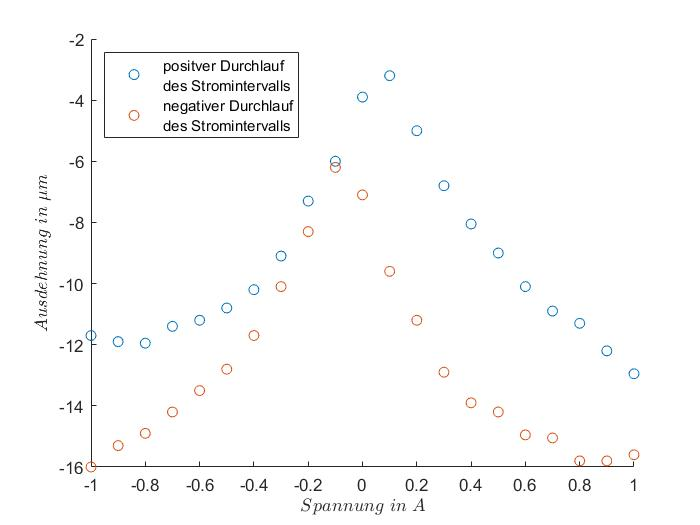
\includegraphics[scale=0.6]{Hysterese des Nickels}\caption{Die hysteresehafte Ausdehnungskurve des Nickelstabs in Abhängigkeit von der Stromstärke}\end{figure}
Dies sind natürlich nicht schöne Kurven wie man sie in der Anleitung zum Skript findet. Aufgrund von physikalischen Veränderungen am Messapparat und womöglich eine ungenaue Justierung der Messuhr gehen hier die Werte nicht nah an 0 wie es eigentlich zu erwarten sei, wenn die Stromstärke selbst bei 0 liegt. Nichtsdestotrotz können wir hier die Steigung mit MATLAB in den Intervallen der Kurven bestimmen in denen die Kurve ansatzweise linear ist. Wir erhalten für die Steigungen die Werte 
\begin{table}[H]
\begin{tabular}[h]{p{3.5cm}|p{3.5cm}|p{3.5cm}|p{3.5cm}}
ansteigende Flanke der positiven \newline{Richtung}&abfallende Flanke der positiven Richtung &abfallende Flanke der negativen Richtung&ansteigende Flanke der negativen \newline{Richtung} \\
\hline
 16,9 $\frac{\mu\textrm{m}}{A}$ & -15,25$\frac{\mu\textrm{m}}{A}$ & 17,0$\frac{\mu\textrm{m}}{A}$ & -16,5 $\frac{\mu\textrm{m}}{A}$  \\
\end{tabular}
\caption{Steigungswerte für die verschiedenen Kurvenabschnitte}
\end{table}
Wir bilden den Mittelwert und den statistischen Fehler. Dabei nehmen wir hier jetzt nur die Beträge der Steigungen.  
\begin{align*}
\overline{m} = (16,4125 \pm 0,4023)\frac{\mu\textrm{m}}{A}
\end{align*}
Weiter interessieren wir uns für die Magnetostriktionskonstante $\kappa \Gamma$. Diese erhalten wir durch Gleichung (14). 
\begin{align*}
\kappa \Gamma = \frac{\overline{m}EL}{N \ell}
\end{align*}
Der Fehler pflanzt sich auch hier wieder fort und man erhält mit den Größen $N=5390$, $L=39,7$cm, $\ell = 44$cm und $E=210$GPa das Ergebnis 
\begin{align*}
\kappa \Gamma \approx ( 576,95 \pm 14,14 ) \frac{\textrm{N}}{\textrm{Am}} 
\end{align*}
Dies kommt sehr grob an die 500 $\frac{\textrm{N}}{\textrm{Am}}$ heran die in der Anleitung zum Versuch erwähnt wurde. Die maximale relative Längenänderung ermitteln wir leicht aus unseren Messwerten. Sie betrug 
\begin{align*}
\frac{\Delta \ell}{\ell} = 36,36 \frac{\mu \textrm{m}}{\textrm{m}}
\end{align*}
Dieser Wert überschreitet nicht die 40$\frac{\mu \textrm{m}}{\textrm{m}}$ die in der Anleitung zum Versuch erwähnt wurde, was so sein sollte. 


\newpage

\subsection{Auswertung 3}
Weiter präsentieren wir einen Plot der die Situation in \glqq Versuch 3\grqq \space etwas wiederspiegelt. 
\begin{figure}[H]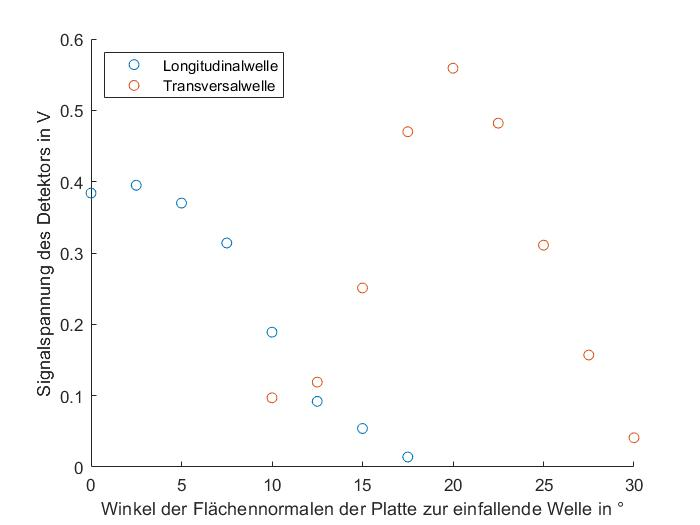
\includegraphics[scale=0.6]{Schallwellen durch Platte}\caption{Die zur Intensität verwandte aufgezeichnete Spannung am Detektor. Es wurden somit die Intensitätsverläufe des sich longitudinal und transversal fortpflanzenden Anteils der auf die Platte auftreffenden Wellen in Abhängigkeit zum Auftreffwinkel gemessen.}\end{figure}
Zu sehen ist, dass ungefähr die Transversalwelle ab einen Winkel von $10^\circ$ auftaucht und die Longitudinalwelle ab dem Winkel $17,5^\circ$ verschwindet. Bei $20^\circ$ ist die Transversalwelle ungefähr maximal. Also haben wir $\alpha_\textrm{L}$ und $\alpha_{T}$ abgelesen ( $\alpha_\textrm{L} = 13^\circ$ und $\alpha_\textrm{T}= 20^\circ$ ), wobei wir den verfälschten Verlauf des Endstücks der Kurve für die Longitudinalwelle ignorierten, und den Nullpunkt bei einem linearen Endverlauf mit dem Auge abschätzten. Wir schätzen ihre systematische Unsicherheit auf $\pm 1,5^\circ$. Zuallererst berechnen wir die Schallgeschwindigkeiten mit den Gleichungen in (17). Wir benutzen dazu $c_\textrm{W}=1480\frac{\textrm{m}}{\textrm{s}}$. Dann erhält man mit Fehlerfortpflanzung
\begin{align*}
c_\textrm{L} = 6579.2 \frac{\textrm{m}}{\textrm{s}} \pm 746.1 \frac{\textrm{m}}{\textrm{s}} \qquad \qquad c_\textrm{T} = 3059.8  \frac{\textrm{m}}{\textrm{s}} \pm 220.1 \frac{\textrm{m}}{\textrm{s}}
\end{align*}
Die auf Wikipedia angegeben Werte für die Schallgeschwindigkeiten bei 20°C betragen $c_L=6250-6350\,\frac{m}{s}$ und $c_T=3100\,\frac{m}{s}$, was durch den Fehlerbereich unserer gemessenen Werte gut getroffen wird. Analog geht es weiter mit dem Elastizitätsmodul $E\approx \rho c_\textrm{L}^2$, mit $\rho = 2,7\frac{\textrm{g}}{\textrm{cm}^3}$ erhalten wir
\begin{align*}
E = 116.87 \textrm{GPa} \pm 26.51 \textrm{GPa}
\end{align*}
Wikipedia gibt diesen Wert auf 70GPa bei 20°C an. Diese deutliche Abweichung, ist aufgrund des Umstand, dass unser Wert für die Schallgeschwindigkeit ziemlich genau war, nur damit zu erklären, dass die Formel in der Anleitung eine großzügige Approximation ist. Als nächstes wird der Schubmodul bestimmt über $G=\rho c_\textrm{T}^2$. 
\begin{align*}
G = 25.28 \textrm{GPa} \pm 3.64 \textrm{GPa}
\end{align*}
Der von Wikipedia angegebene Wert von 25,5 GPa bei Raumtemperatur liegt jetzt viel näher an unserem Wert. Der Grund dafür ist wieder in einer wohl genauern Approximation bei der verwendeten Formel zu suchen. Weiter machen wir mit der Querkontraktionszahl und nutzen dabei Gleichung (19). Wir erhalten 
\begin{align*}
\nu = 0.3620 \pm 0.0473 
\end{align*}
Auch hierbei treffen wir den von Wikipedia auf 0.35 angegebenen Wert erfreulich gut.
\newpage
\section{Fazit}
Wir konnten in diesen drei Versuchen vieles über Schallwellen und ihre Ausbreitung in Festkörpern, Gasen und Flüssigkeiten lernen. Die Versuchsergebnisse waren größtenteils in einem akzeptablen Bereich, auch wenn manche Werte etwas daneben lagen. Alles im allem, konnten wir uns von der Gültigkeit der vorhandenen Theorie über Ultraschallwellen überzeugen.












\end{document}